%Template by Morten Espensen
%Deffinere kommandoer til om vores information

\documentclass[]{report}
%\usepackage{color}
%\usepackage{alltt}
\usepackage{amsmath}
\usepackage{amssymb}
\usepackage{float}
\usepackage[parfill]{parskip}
\usepackage{lscape}
\usepackage{enumerate}
\usepackage{amsmath}
\usepackage[danish,english]{babel}

\usepackage[paper=A4,pagesize]{typearea}
\usepackage[toc,page]{appendix}

\usepackage[utf8]{inputenc}
\usepackage{fancyhdr}
%\usepackage{boxproof}
%\usepackage{daymonthyear}
\usepackage{stmaryrd}

\usepackage{color}
\usepackage{fancyvrb}
\usepackage[usenames,dvipsnames]{xcolor}
\fvset{frame=single,framesep=1mm,fontfamily=courier,fontsize=\scriptsize,numbers=left,framerule=.3mm,numbersep=1mm,commandchars=\\\{\}}

\usepackage{wallpaper} % For the frontpage background

\usepackage{listings} % KODE SHIT
\lstset{ %
language=PHP,          		    % the language of the code
basicstyle=\footnotesize,       % the size of the fonts that are used for the code
numbers=left,                   % where to put the line-numbers
numberstyle=\footnotesize,      % the size of the fonts that are used for the line-numbers
stepnumber=1,                   % the step between two line-numbers. If it's 1, each line
                                % will be numbered
numbersep=5pt,                  % how far the line-numbers are from the code
backgroundcolor=\color{white},  % choose the background color. You must add \usepackage{color}
showspaces=false,               % show spaces adding particular underscores
showstringspaces=false,         % underline spaces within strings
showtabs=false,                 % show tabs within strings adding particular underscores
frame=single,                   % adds a frame around the code
tabsize=2,                      % sets default tabsize to 2 spaces
captionpos=b,                   % sets the caption-position to bottom
breaklines=true,                % sets automatic line breaking
breakatwhitespace=false,        % sets if automatic breaks should only happen at whitespace
title=\lstname,                 % show the filename of files included with \lstinputlisting;
                                % also try caption instead of title
escapeinside={\%*}{*)},         % if you want to add a comment within your code
morekeywords={*,...,xchar,xstring,xmany1,chainl1,chainl1',ReadP}            % if you want to add more keywords to the set
}

\newcommand{\theassingment}{Development of E-learning concept\\[1.6ex]for Medical Personnel}
\newcommand{\thesubassignment}{Strategic Alignment Report}
\newcommand{\shorttheassingment}{ITIC}
%\newcommand{\thepaperauthor}{}
\newcommand{\personalid}{dzr440 - 19/06/1991}
\newcommand{\thesubject}{IT Innovation and Change}
\newcommand{\theinstitute}{Department of Computer Science}
\newcommand{\thesupervisor}{Cosmin E. Oancea} %behøves kun hvis findes

\newcommand*{\diffdchar}{\mathrm{d}}    % or {ⅆ}, or {\mathrm{d}}, or whatever standard you’d like to adhere to
\newcommand*{\dd}{\mathop{\diffdchar\!}}

\newenvironment{timesfont}{\fontfamily{mathptmx}\selectfont}{}

\setlength\parskip{2ex}
\newcommand{\n}[0]{\\[2ex]} %NEWLINE [2ex]
\newcommand{\set}[1]{\{#1\}}
\usepackage{hyperref}

\newcommand{\fnurl}[2]{\href{#2}{#1}\footnote{\url{#2}}}  %foodnote url ref \fnurl{String}{Link}

\newcommand{\premise}{\=\mbox{premise}}
\newcommand{\assumption}{\=\mbox{assumption}}
\newcommand{\landi}{\=\intro\land : }
\newcommand{\lande}{\=\elim\land_{1} : }
\newcommand{\landee}{\=\elim\land_{2} : }
\newcommand{\lori}{\=\intro\lor_{1} : }
\newcommand{\lorii}{\=\intro\lor_{2} : }
\newcommand{\lore}{\=\elim\lor : }
\newcommand{\toi}{\=\intro\to : }
\newcommand{\toe}{\=\elim\to : }
\newcommand{\lnoti}{\=\intro\lnot : }
\newcommand{\lnote}{\=\elim\lnot : }
\newcommand{\bote}{\=\elim\bot : }
\newcommand{\lnege}{\=\lnot\elim\lnot : }
\newcommand{\lnegi}{\=\lnot\intro\lnot : }
\newcommand{\leqi}{\= \intro= }
\newcommand{\leqe}{\= \elim= : }
\newcommand{\lforalli}{\= \intro\forall : }
\newcommand{\lforalle}{\= \elim\forall : }
\newcommand{\lexistsi}{\= \intro\exists : }
\newcommand{\lexistse}{\= \elim\exists : }
\newcommand{\MT}{\=MT : }
\newcommand{\PBC}{\=PBC : }
\newcommand{\LEM}{\=LEM : }

\newenvironment{changemargin}[1]{
  \begin{list}{}{
    \setlength{\voffset}{#1}
  }
  \item[]}{\end{list}}


\usepackage{hyperref}
\usepackage{pdfpages} % til at tilføje apendix
\usepackage{graphicx}
\DeclareGraphicsExtensions{.pdf,.png,.jpg}

\def\thesection{\thechapter.\arabic{section}}
%\renewcommand{\thesubsection} {\thesection.\alph{subsection}}

\pagestyle{fancy}
\fancyhead{}
\fancyhead[LO,LE]{\shorttheassingment}
\fancyhead[RO,RE]{\today}
\fancyhead[CO,CE]{\theinstitute}

\setcounter{secnumdepth}{0}
\setcounter{tocdepth}{3}

\begin{document}
\begin{titlepage}
\begin{timesfont}
% Import the ku frontpage graphics
\ThisULCornerWallPaper{1}{nat-farve.pdf}
% Import faculty title
\ThisULCornerWallPaper{1}{nat-en.pdf}
% For forklaring af vspace og stretch, se side 115 i ".. not so short .."
% www.ctan.org/tex-archive/info/lshort/english/lshort.pdf
\vspace*{3cm}
\hspace*{-2.3cm}
% Her vælger en kæmpe skrifttype og fed skrift
\Huge\bfseries
\vspace*{-0.5cm}
\theassingment\n
\hspace*{-2.4cm}
-- \thesubassignment \n
\LARGE
\hspace*{-2.4cm}
\vspace*{-0.5cm}
\thesubject \\[2.2ex]
\hspace*{-2.4cm}
\vspace*{5.0cm}
\theinstitute \n
\hspace*{-2.38cm}
\large
\textbf{Written by:}\\[1ex]
\hspace*{-2.33cm}
Morten Espensen (dzr440)\\
\hspace*{-2.33cm}
David B. Gandrup (vpd177)\\
\hspace*{-2.33cm}
Sokratis S. Drosos (dnb823)\\
\hspace*{-2.33cm}
Bjarki Madsen (lch929)\\
\hspace*{-2.33cm}
Niklas Høj (nwv762)\\
%\vspace*{1cm}
\hspace*{-2.33cm}
% Nulstiller skriftstørrelse og type (f.eks. fed)
\normalsize
% VEJLEDER INFORMATION I PÅ FORSIDEN?
%\thesubject \n

\hspace*{-2.33cm}
%\textbf{\emph{Supervised by:}}

\hspace*{-2.33cm}
%\thesupervisor

\end{timesfont}
\end{titlepage}
\tableofcontents

\newpage

\section{Approach}
In our inline analysis phase we have conducted an initial interview with a representative of DMA and created a baseline plan. After completing the baseline plan, we performed document analysis in order to narrow our scope and research current e-learning solutions.

After this initial phase we went on to having a company visit at DMA and meeting with the representative of DMA. At the meeting we performed scope identification, functional analysis, identified possible stakeholders, contact persons and possible steering committee members. Accordingly we discussed further material that would be relevant to research to narrow our scope further.

Based on the meeting with the DMA representative we performed additional document analysis along with functional analysis.

\section{Environment}
The Danish Medical Association (DMA) is an association that aims to represent the entire Danish medical sector and its existing organisations, tying them all together and providing benefits for all its members. There are three major medical organisations under the DMA. The structure is illustrated in figure \ref{dmaorganisation}.

The first is “Yngre Læger” (YL), an association for younger doctors with close ties to doctors advancing their studies in the “klinisk basisuddannelse” (KBU), those taking their introduction to their speciality and those who are actively specialising.

The second is “Forening af Speciallæger” (FAS) which is a union for consulting doctors that have studied a speciality.

Lastly is “Praktiserende Lægers Organisation” (PLO) which is an organisation for the practicioning family doctors who usually run their own local clinic for the nearby population.

Danish doctors are generally associated with one of these three organisations and are thus members of the DMA, having access to the DMA provided courses and other benefits.

\begin{figure*}[h!]
 \begin{center}
  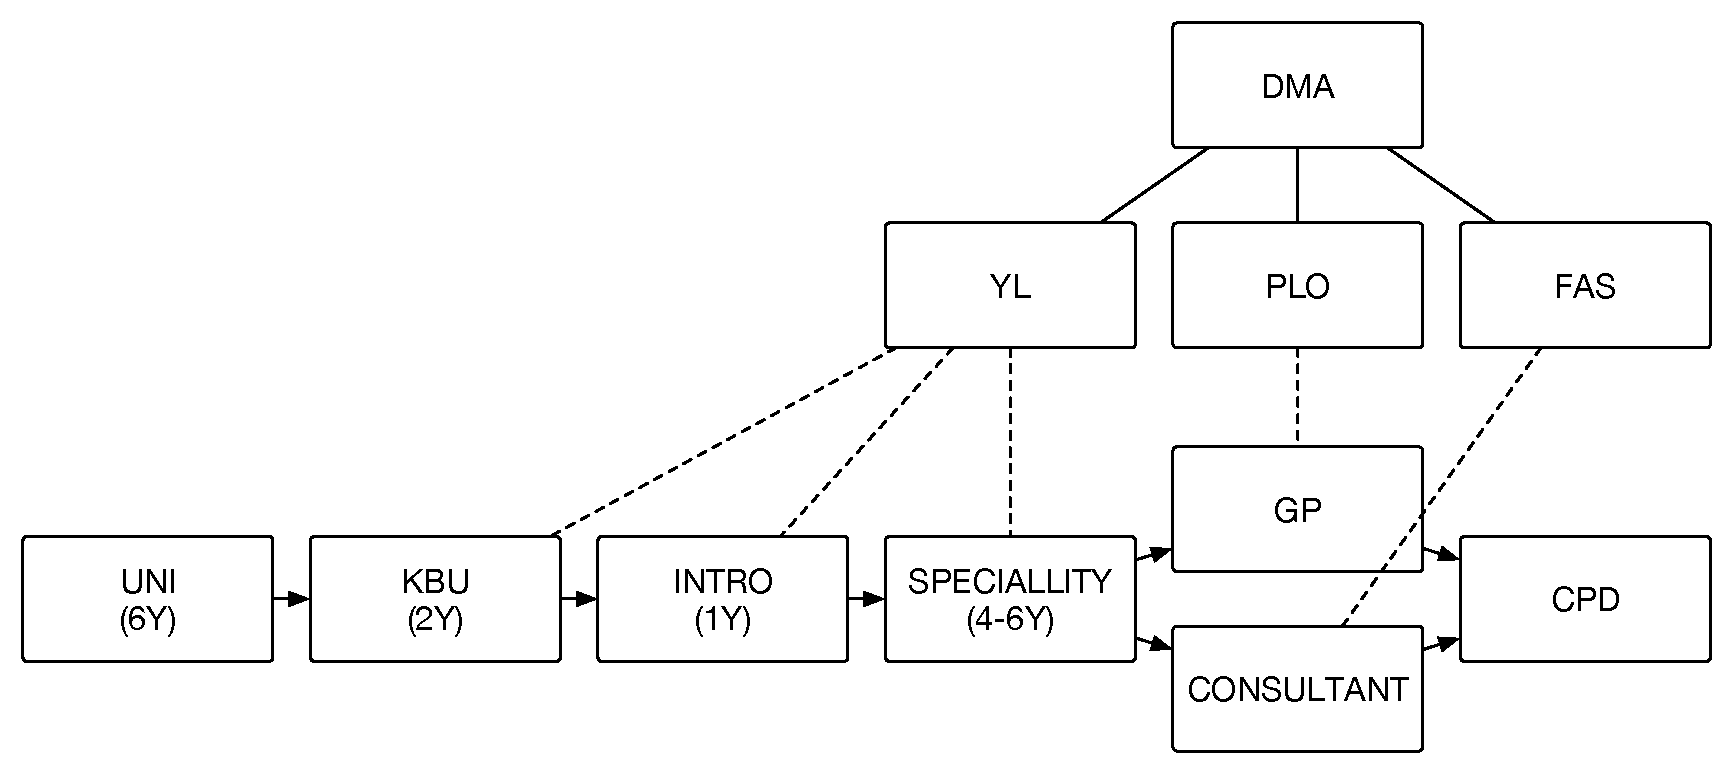
\includegraphics[width=1\textwidth]{figures/dma-structure.pdf}
  \caption{The structure of the DMA organisation.\label{dmaorganisation}}
 \end{center}
\end{figure*}

\subsection{Potential and needs}
DMA members need to take courses in order to stay up to date with the latest information about medicine. So far the existing e-learning platforms that provide the necessary courses are not widely used by the doctors, in some cases this is because they consider it to be time consuming. Some doctors also consider the contents of the e-learning courses to be too easy and superficial.. What is needed is a new way to deliver information to the doctors, such that we can engage the doctors in a way that eliminates the concerns of the current e-learning solutions.

\subsection{Requirements and conditions}
DMA members are looking for a new e-learning platform with a different approach compared to the existing offers provided by DMA, such as BMJ Learning as the DMA members currently do not utilise the offers as much as expected. DMA would like to have the content focused on including the entire spectrum (known as the 7 roles of physicians) of knowledge areas which a modern doctor should be educated in, for example there should be topics dealing with communication, administration and so on. Currently surveys performed by DMA show that some doctors prefer to strictly focus their education on medical expertise and entirely neglecting being educated in the remaining 6 roles.

\subsection{Special conditions}
We do not identify any special conditions at this point.


\section{Business strategy}
\subsection{Goals}
In the end, we aim to find an approach for doctors to learn course material that will work for the busy doctors. The approach should be realistic and feasible within the constraints of the target association DMA, and should actually engage the doctors and fit their needs so that the doctors will use it in practise.

\subsection{Business processes}
We do not consider business processes relevant at this time, as it is outside the scope of our study.

\subsection{Challenges and problems}
There are various challenges associated with solving the problem of doctors not actively continuing their education despite attempts to facilitate their learning. Firstly, we need to establish what is actually causing the problem. The cause seems to be that the doctors do not have time in their busy schedules to take hours or entire days off to study and take courses, but is this actually the main cause? Is there more to it? Are other factors in the way of doctors keeping up with their fields?

If the stated problem is confirmed to be what it seems to be, then we still have the problem of figuring out an alternative method of providing the course materials in a manner that is accessible to the doctors. And even with accessible learning, the approach still needs to motivate the doctors to actually use the solution. So we need to understand exactly what the doctors are looking for in a way of consuming courses and exactly what will suit their needs.

\section{Work domains}
We have identified two primary work domains: Course creation and Doctors practice.

\subsection{Course creation}
\subsubsection{Definition}
The course creation work domain is the source that DMA uses to provide material for their members to educate themselves. It is not limited to the creators that DMA are directly linked with, but also external third party creators.

\subsubsection{Characterization}
DMA has multiple sources of courses and material of differing types and they are delivered in different ways, from BMJ’s e-learning platform, DMA’s own courses and courses created elsewhere and communicated to members through and by DMA.

The sources have different delivery methods, course content, evaluation methods and purpose.

DMA primarily uses their website and other IT based channels to inform their members of the existence of these courses, and to some extent also give access to them.

\subsubsection{Discussion/conclusion}
The constraints and methods in course creation are key to determining what is possible to actually do in terms of innovative ideas.

\subsection{Doctors practice}
\subsubsection{Definition}
The actual work practice and daily schedule of DMA’s members, the doctors, and how much time and resources they have available for learning new things. This means both considering the day to day work schedule and any time dedicated to learning.

\subsubsection{Characterization}
Although DMA serves a very diverse member group, there is some common ground and work practices among a large part of their members. The doctors have a busy working day that is not very flexible, making it difficult for them to make time for the current format of provided courses.

Additionally some members lack incentive to prioritise learning over working, as some doctors are paid to learn, others are not.

\subsubsection{Discussion/conclusion}
Whatever the quality of the courses provided by DMA may be, the doctors have to be able to find the time to take them. The courses also need to cater for the actual interests of the doctors and be relevant in their daily work.


\section{Scope}
The focus of our in-depth analysis phase will be to investigate exactly how the course creation works and what the limitations and possibilities are, and what kind of learning format would actually fit into the doctors’ schedule. The goal is to find out exactly how and where to focus our efforts to help the course creators model their content so the doctors will want to and be able to use it.

We consider our project to be either a situation 3 or 4, as described in Bødker, Kensing & Simonsen (2004), page 142, currently more a 4 than 3. We have limited knowledge of the actual structure of the work domains, and the organization and the amount of interest groups is quite high, putting us in a situation 4. This might change as we narrow our focus though, especially in regards to which course creators we ultimately ending up working with.
We need to gather more data on the work practices in our primary work domains and analyse them to focus our project.

\section{Business model canvas}
\begin{figure*}
 \begin{center}
  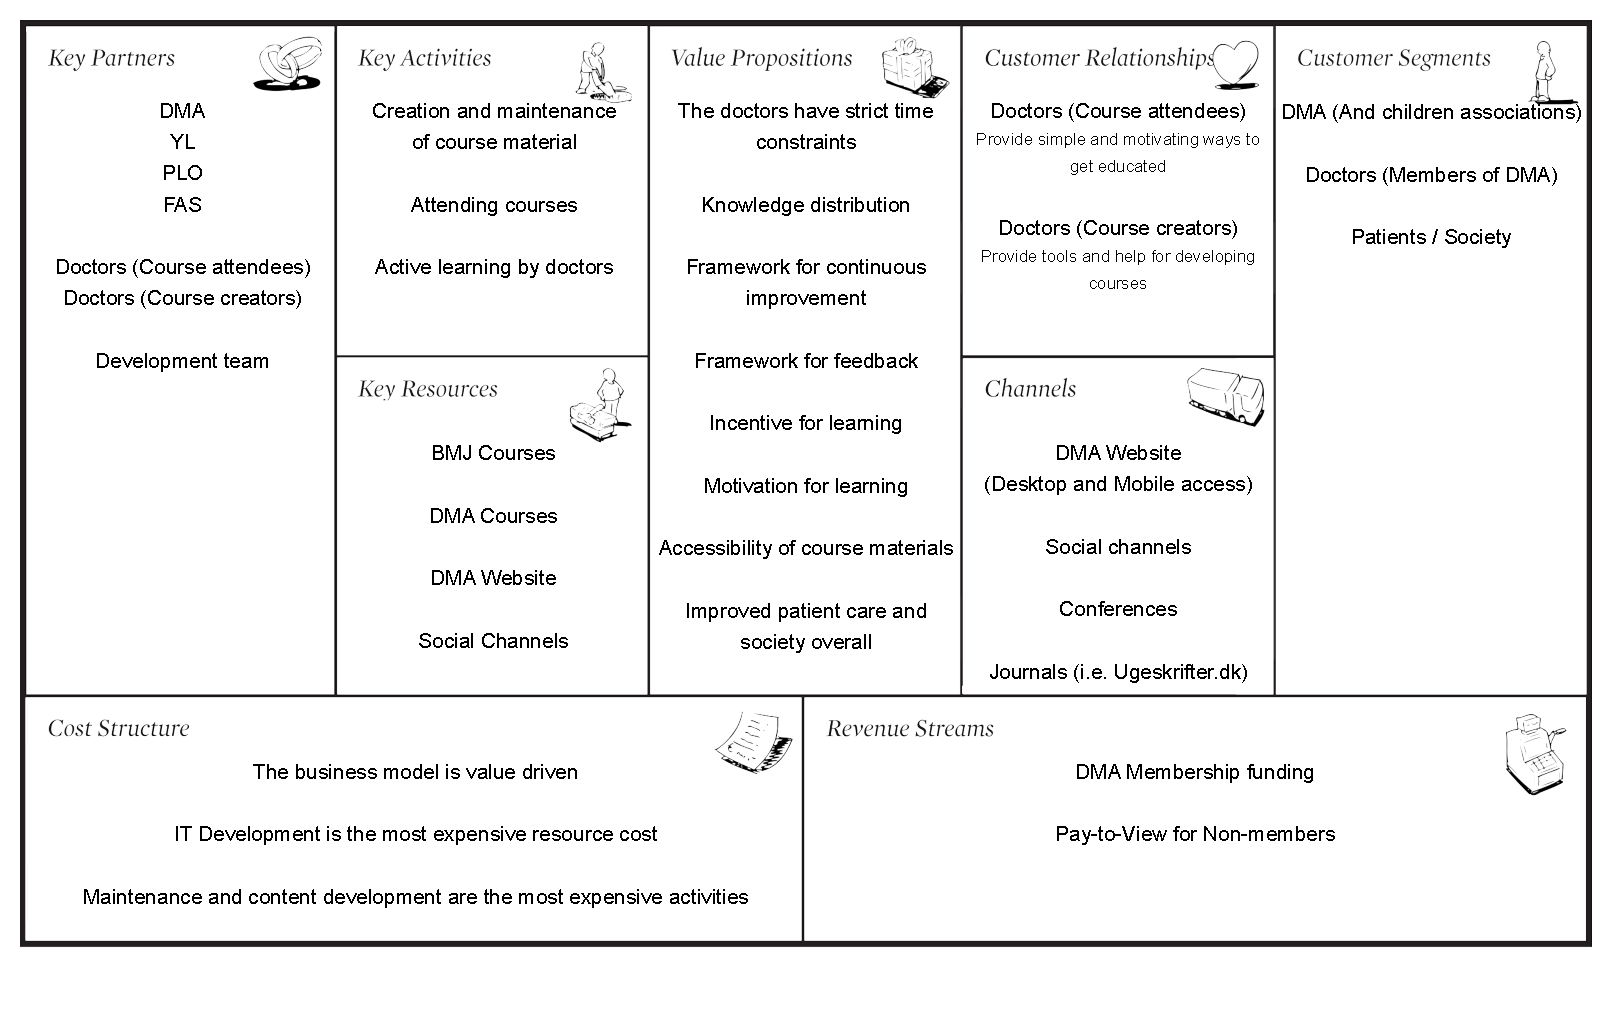
\includegraphics[width=1\textwidth]{figures/business-model-canvas.pdf}
  \caption{Our baseline plan for the project.\label{dmaorganisation}}
 \end{center}
\end{figure*}




\end{document}
